\subsection{MSVC + \olly}
\myindex{\olly}
Let's illustrate this in \olly.
When we trace to the first instruction in \ttf that uses one of the arguments 
(first one), we see that \EBP is pointing to the \gls{stack frame}, 
which is marked with a red rectangle.

The first element of the \gls{stack frame} is the saved value of \EBP, 
the second one is \ac{RA}, the third is the first function argument, then the second and third ones.

To access the first function argument, one needs to add exactly 8 (2 32-bit words) to \EBP.

\olly is aware about this, so it has added comments to the stack elements like

\q{RETURN from} and \q{Arg1 = \dots}, etc.

N.B.: Function arguments are not members of the function's stack frame, they are rather
members of the stack frame of the \gls{caller} function.

Hence, \olly marked \q{Arg} elements as members of another stack frame.

\begin{figure}[H]
\centering
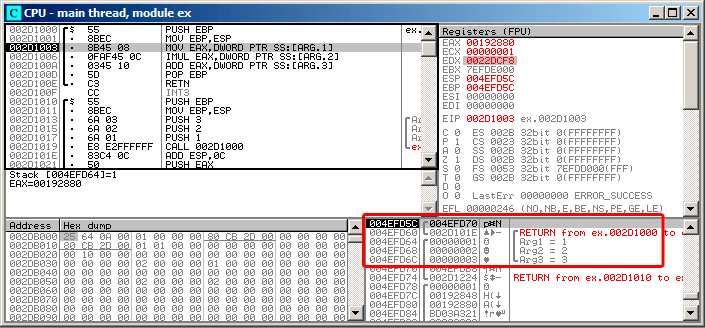
\includegraphics[scale=\FigScale]{patterns/05_passing_arguments/olly.png}
\caption{\olly: inside of \ttf{} function}
\label{fig:passing_arguments_olly}
\end{figure}

